% !TeX encoding = UTF-8
% !TeX program = xelatex
% !TeX spellcheck = en_US

\documentclass[degree=project, degree-type=project]{thuthesis}
\usepackage{mathtools}
% Syntax Highlighting in LaTeX, need pygments
% Must build with xelatex -shell-escape -enable-8bit-chars.
\usepackage{minted}
% https://tex.stackexchange.com/a/112573
\usepackage{tcolorbox}
\usepackage{etoolbox}
\BeforeBeginEnvironment{minted}{\begin{tcolorbox}}%
\AfterEndEnvironment{minted}{\end{tcolorbox}}%
% color for minted
\definecolor{friendlybg}{HTML}{f0f0f0}


% 论文基本配置,加载宏包等全局配置
\thusetup{
    output = electronic,
    title  = {实验二:矩阵分解},
    author  = {肖文韬},
    studentid = {2020214245},
    course = {大数据分析},
    include-spine = false,
}

\usepackage{float}
\usepackage[sort]{natbib}
\bibliographystyle{thuthesis-numeric}
\graphicspath{{figures/}}


\begin{document}

% 封面
\maketitle

\frontmatter
% % !TeX root = ../thuthesis-example.tex

% 中英文摘要和关键字

\begin{abstract}
  论文的摘要是对论文研究内容和成果的高度概括。摘要应对论文所研究的问题及其研究目
  的进行描述,对研究方法和过程进行简单介绍,对研究成果和所得结论进行概括。摘要应
  具有独立性和自明性,其内容应包含与论文全文同等量的主要信息。使读者即使不阅读全
  文,通过摘要就能了解论文的总体内容和主要成果。

  论文摘要的书写应力求精确、简明。切忌写成对论文书写内容进行提要的形式,尤其要避
  免“第 1 章……;第 2 章……;……”这种或类似的陈述方式。

  本文介绍清华大学论文模板 \thuthesis{} 的使用方法。本模板符合学校的本科、硕士、
  博士论文格式要求。

  本文的创新点主要有:
  \begin{itemize}
    \item 用例子来解释模板的使用方法;
    \item 用废话来填充无关紧要的部分;
    \item 一边学习摸索一边编写新代码。
  \end{itemize}

  关键词是为了文献标引工作、用以表示全文主要内容信息的单词或术语。关键词不超过 5
  个,每个关键词中间用分号分隔。(模板作者注:关键词分隔符不用考虑,模板会自动处
  理。英文关键词同理。)

  % 关键词用“英文逗号”分隔
  \thusetup{
    keywords = {TeX, LaTeX, CJK, 模板, 论文},
  }
\end{abstract}

\begin{abstract*}
  An abstract of a dissertation is a summary and extraction of research work
  and contributions. Included in an abstract should be description of research
  topic and research objective, brief introduction to methodology and research
  process, and summarization of conclusion and contributions of the
  research. An abstract should be characterized by independence and clarity and
  carry identical information with the dissertation. It should be such that the
  general idea and major contributions of the dissertation are conveyed without
  reading the dissertation.

  An abstract should be concise and to the point. It is a misunderstanding to
  make an abstract an outline of the dissertation and words ``the first
  chapter'', ``the second chapter'' and the like should be avoided in the
  abstract.

  Key words are terms used in a dissertation for indexing, reflecting core
  information of the dissertation. An abstract may contain a maximum of 5 key
  words, with semi-colons used in between to separate one another.

  \thusetup{
    keywords* = {TeX, LaTeX, CJK, template, thesis},
  }
\end{abstract*}


% 目录
\tableofcontents

% 正文部分
\mainmatter

\chapter{数据整理}

数据集每一行为 \texttt{<user\_id> <movie\_id> <rate>} 的格式:

\begin{enumerate}
  \item user\_id: 用户唯一 id,用户数量为 $10000$,不过用户 id 并不在 $[0, 10000]$ 内,需要自己创建一个 user2id 的映射。
  \item movie\_id: 电影唯一 id,电影数量为 $10000$,并且电影 id $\in [1, 10001]$。
  \item rate: 电影打分,为 $[0, 5]$ 的整数,其中 $0$ 表示未打分。
\end{enumerate}

观察分析数据后,有以下结论:

\begin{enumerate}
  \item 训练集和测试集中的数据并不是规整的按电影来划分的,也就是说对于某个电影,训练集和测试集都只有一部分用户打分。并且打分是不重叠的,也就是说如果用户在训练集中打了分,在测试集中就是没打分的,反之亦然。
  \item 因为数据规模不是很大,矩阵虽然是 $10000 \times 10000$ 大小的,不过比较稀疏(训练集稀疏度 6.89\%,测试集 1.72\%),所以可以使用稀疏矩阵来加快速度。
\end{enumerate}

总之,该数据集不算很大,合理使用稀疏矩阵,使用矩阵运算(并行)来代替循环,在显卡上进行矩阵运算,都可以大大的提高处理速度。

\textbf{故在实验中,采用全量数据。}

数据读取部分的代码实现:

  \begin{minted}[texcomments,tabsize=2,style=friendly,bgcolor=friendlybg]{python}
def read_data(filename):
  user2id = {}
  st = time()
  X = np.zeros((10000, 10000))
  with open(filename) as f:
    for l in f.readlines():
      user, movie, rate, _ = l.split()
      movie = int(movie) - 1
      rate = int(rate)
      if user not in user2id:
        user2id[user] = len(user2id)
      user = user2id[user]
      X[user, movie] = rate
  print(f'Done in {time() - st}s.')
  return X

X_train = read_data('netflix_train.txt')
X_test = read_data('netflix_test.txt')')
  \end{minted}

\chapter{任务一:协同过滤算法}

协同过滤(Collaborative Filtering)是一种经典的且被工业界广泛使用推荐算法。
狭义的协同过滤定义为:通过收集大量其他\textbf{相似}用户的偏好或品味信息(\textbf{协同})来自动地对预测(\textbf{过滤})当前用户的兴趣。
广义的协同过滤则定义为:使用多个主体,观点,数据源进行合作来过滤信息或者模式的过程。

协同过滤算法分为两类:

\begin{enumerate}
  \item 基于用户的协同过滤:构建一个 user-item 矩阵,然后寻找该用户的相似用户在 user-item 矩阵中的信息来预测该用户的偏好结果。
  \item 基于目标项目(item)的协同过滤:构建一个 item-item 矩阵来衡量不同项目之间的关联度,然后使用该矩阵来推导用户的偏好。
\end{enumerate}

这里主要是实现一个基于用户的协同过滤算法,基于用户的协同过滤算法的一般定义为(用户 $i$ 对项目 $m$ 的打分):
\begin{equation}
  score(i, m) = \text{agg}_{j \in N}(score(j, m))
\end{equation}

其中 $N$ 表示 $i$ 的某个邻域(一般以相似度作为度量),$agg$ 用户对该邻域内所有打分结果进行聚合运算(i.e., 加权平均),包括一些预处理(归一化,收缩,等)。

本节将要实现的算法的核心公式为(以预测用户 $i$ 对电影 $m$ 的偏好度为例):
\begin{equation}
score(i, m) = \frac{\sum_{k \in N(i, m)} sim(X(i), X(k)) \times score(k, m)}{\sum_{k \in N(i, m)} sim(X(i), X(k))}
  \label{coll_filter}
\end{equation}

其中 $X(i)$ 代表用户 $i$ 对所有电影的打分(当然要预测的电影的打分是为 0 的)向量,$N(i, m)$ 在本例中简单选用为所有给电影 $m$ 打了分的用户,相似度量采用\textbf{余弦距离(cosine distance)}:
\begin{equation}
sim(X(i), X(k)) = \frac{\langle X(i), X(k) \rangle}{\lVert X(i) \rVert \lVert X(k) \rVert}
\end{equation}

公式 \ref{coll_filter} 可以转换为矩阵运算的形式:
\begin{align}
  \begin{split}
    \hat{X} = \frac{S \cdot X}{S \cdot A}
  \end{split}
\end{align}
其中 $A$ 为 $X$ 的指示矩阵,有 $A_{ij} = \text{sgn}(X_{ij})$,$S$ 是相似度矩阵。

在 Python 上使用 numpy 实现的代码为:

  \begin{minted}[texcomments,tabsize=2,style=friendly,bgcolor=friendlybg]{python}
def pairwise_cos_distance(X):
  X = X.T / X.sum(axis=1)
  return X.T @ X

def coll_filter_sp(train: np.ndarray):
  sim = pairwise_cos_distance(train)
  score = sim @ train
  train = train.astype(np.bool)
  Z = sim @ train
  return score_pred
  \end{minted}

虽然转换成矩阵运算之后,相对于简单粗暴的 for 循环实现,速度上已经有了很明显的提升。不过既然是矩阵运算,理说应当更加适合在显卡上进行运算。
以下是使用 cupy\footnote{一个类似于 numpy 的矩阵运算库,不过所有运算都是在 GPU 上进行的。} 实现的版本(是的,基本上就是把 \texttt{np} 改成了 \texttt{cp})。

  \begin{minted}[texcomments,tabsize=2,style=friendly,bgcolor=friendlybg]{python}
def coll_filter_cuda(train: cp.ndarray):
  cp.cuda.Device(3).use()
  X_train_cuda = cp.array(train)
  X_test_cuda = cp.array(test)
  sim = pairwise_cos_distance(X_train_cuda)
  score = sim @ X_train_cuda
  Z = sim @ X_train_cuda.astype(np.bool)
  score_pred = score / Z
  return score_pred
  \end{minted}

RMSE 因为测试样本数不是 $10000 * 10000$ 而是 170 多万,所以最好不要使用 numpy 提供的 RMSE,我们可以自己简单实现一下:

  \begin{minted}[texcomments,tabsize=2,style=friendly,bgcolor=friendlybg]{python}
def rmse(X, X_hat):
  test_point = X.astype(np.bool)
  loss = np.sqrt(np.power(
    X_hat[test_point] - X[test_point], 2
  ).mean())
  return loss
  \end{minted}

\begin{table}[htb]
  \centering
  \caption{协同过滤算法不同实现对比}
  \label{table:coll_rmse}
  \begin{tabular}{lll}
    \toprule
    {\heiti 实现} & {\heiti RMSE} & {\heiti 速度(s)} \\\midrule
    CPU & $1.02821$ & $12.94$\\
    CPU ($k$ 取所有) & $2.60669$ &  $7.94$\\
    GPU & $1.02821$ & $11.79$ \\
    GPU ($k$ 取所有) & $2.60669$ & $7.88$ \\
    \bottomrule
  \end{tabular}
\end{table}

最终计算速度和最终的 RMSE 对比如表 \ref{table:coll_rmse}所示。
可以看出,GPU 竟然只比 CPU 快一点点,这样不行呀,至于原因我认为还是因为这里面涉及到一些对 GPU 不太友好的运算(例如归一化用到的两次逐位除法),并且 numpy 优化得比较好了,=,=
总之,在第二个任务,矩阵分解任务,我们就能看到 GPU 运算的魅力啦~

\textbf{备注}:开头说了数据集比较稀疏,可是为什么我最终没有使用稀疏矩阵运算呢?
因为我发现,这个矩阵还是不够大,也不够稀疏,还不如全量矩阵直接用显卡或者 Intel CPU 提供的 AVX 指令集优化地并行加速高效。
使用 scipy 提供的 csr 模式的稀疏矩阵运算大概需要耗时 120s。

\chapter{任务二:矩阵分解算法}

因为给定特征矩阵是一个稀疏矩阵,基于低秩假设,特征维度为 10000 的矩阵的特征值也很稀疏(或者很小),于是我们可以将矩阵分解为两个特征维度很小的隐空间特征表达:
\begin{equation}
X_{m \times n} \approx U_{m \times k} V_{n \times k}^T
\end{equation}
其中 $k \ll n$。

特别的,我们在电影推荐任务中,使用 X\_train 构建出矩阵分解后,使用它们的乘积来预测 X\_test 中的那部分结果。

这里我们采用梯度下降算法来求解上述分解,目标函数为:
\begin{equation}
J = \frac{1}{2} \lVert A \odot (X - UV^T \rVert_F^2 + \lambda \lVert U \rVert_F^2 + \lambda \lVert V \rVert_F^2)
\end{equation}
其中 $\odot$ 表示 Hadamard 乘积(逐位乘),$A$ 为指示矩阵,$A_{ij} = 1$ 表示 $X_{ij}$ 的值已知,$\lVert A \rVert_F^2 = \sqrt{\sum_i \sum_j A_{ij}}$ 表示矩阵 Frobenius 范数,$\lambda$ 为正则化系数,用于防止过拟合。

对目标函数求偏导,得到:
\begin{align}
  \frac{\partial J}{\partial U} &= (A \odot (UV^T - X))V + 2\lambda U\\
  \frac{\partial J}{\partial V} &= (A \odot (UV^T - X))^TU + 2\lambda V
\end{align}

所以整个算法的流程为:

\begin{itemize}
  \item 初始化 $U, V$ 为较小的随机值
  \item 不断循环 $U = U - \alpha \frac{\partial J}{\partial U}, V = V - \alpha \frac{\partial J}{\partial V}$,直到收敛
\end{itemize}

代码实现(CuPy 版本):

  \begin{minted}[texcomments,tabsize=2,fontsize=\footnotesize,style=friendly,bgcolor=friendlybg]{python}
def init_matrix(X, k, n_features=10000,
                n_samples=10000, seed=1234):
  avg = np.sqrt(X.mean() / k)
  rng = np.random.RandomState(seed)
  V = avg * rng.randn(k, n_features).astype(X.dtype, copy=False)
  U = avg * rng.randn(n_samples, k).astype(X.dtype, copy=False)
  np.abs(U, out=U)
  np.abs(V, out=V)
  return cp.array(U), cp.array(V)

def frob_norm_sq(X):
  norm = cp.sum(cp.power(X, 2))
  return norm

def objective(diff, U, V, lamb):
  loss = frob_norm_sq(diff)
  loss = 0.5 * loss + (frob_norm_sq(U) + frob_norm_sq(V)) * lamb
  return loss.item()

def fit(X, k, lamb, alpha=1e-3, tol=1e-4, max_iter=500):
  st_fit = time()
  U, V = init_matrix(X, k)
  A = X.copy()
  A = A.astype(np.bool)
  A = cp.array(A)
  X = cp.array(X)
  prev_error = 0.
  for n_iter in range(1, max_iter + 1):
    diff = A * (U @ V - X)
    update_U = diff @ V.T + 2 * lamb * U
    update_V = U.T @ diff + 2 * lamb * V
    error = objective(-diff, U, V, lamb)
    if n_iter \% 10 == 0:
      print(f'Iter: {n_iter}, loss={error:.4f}, ' +
            f'{(time() - st_fit) / n_iter:.1f}s/epoch.')
    if prev_error != 0 and (prev_error - error) / prev_error <= tol:
      break
    prev_error = error
    U = U - alpha * update_U
    V = V - alpha * update_V
  return U @ V
  \end{minted}

\section{迭代过程}

\begin{figure}[h]
\centering%
\subcaptionbox{训练损失值\label{fig:loss}}
{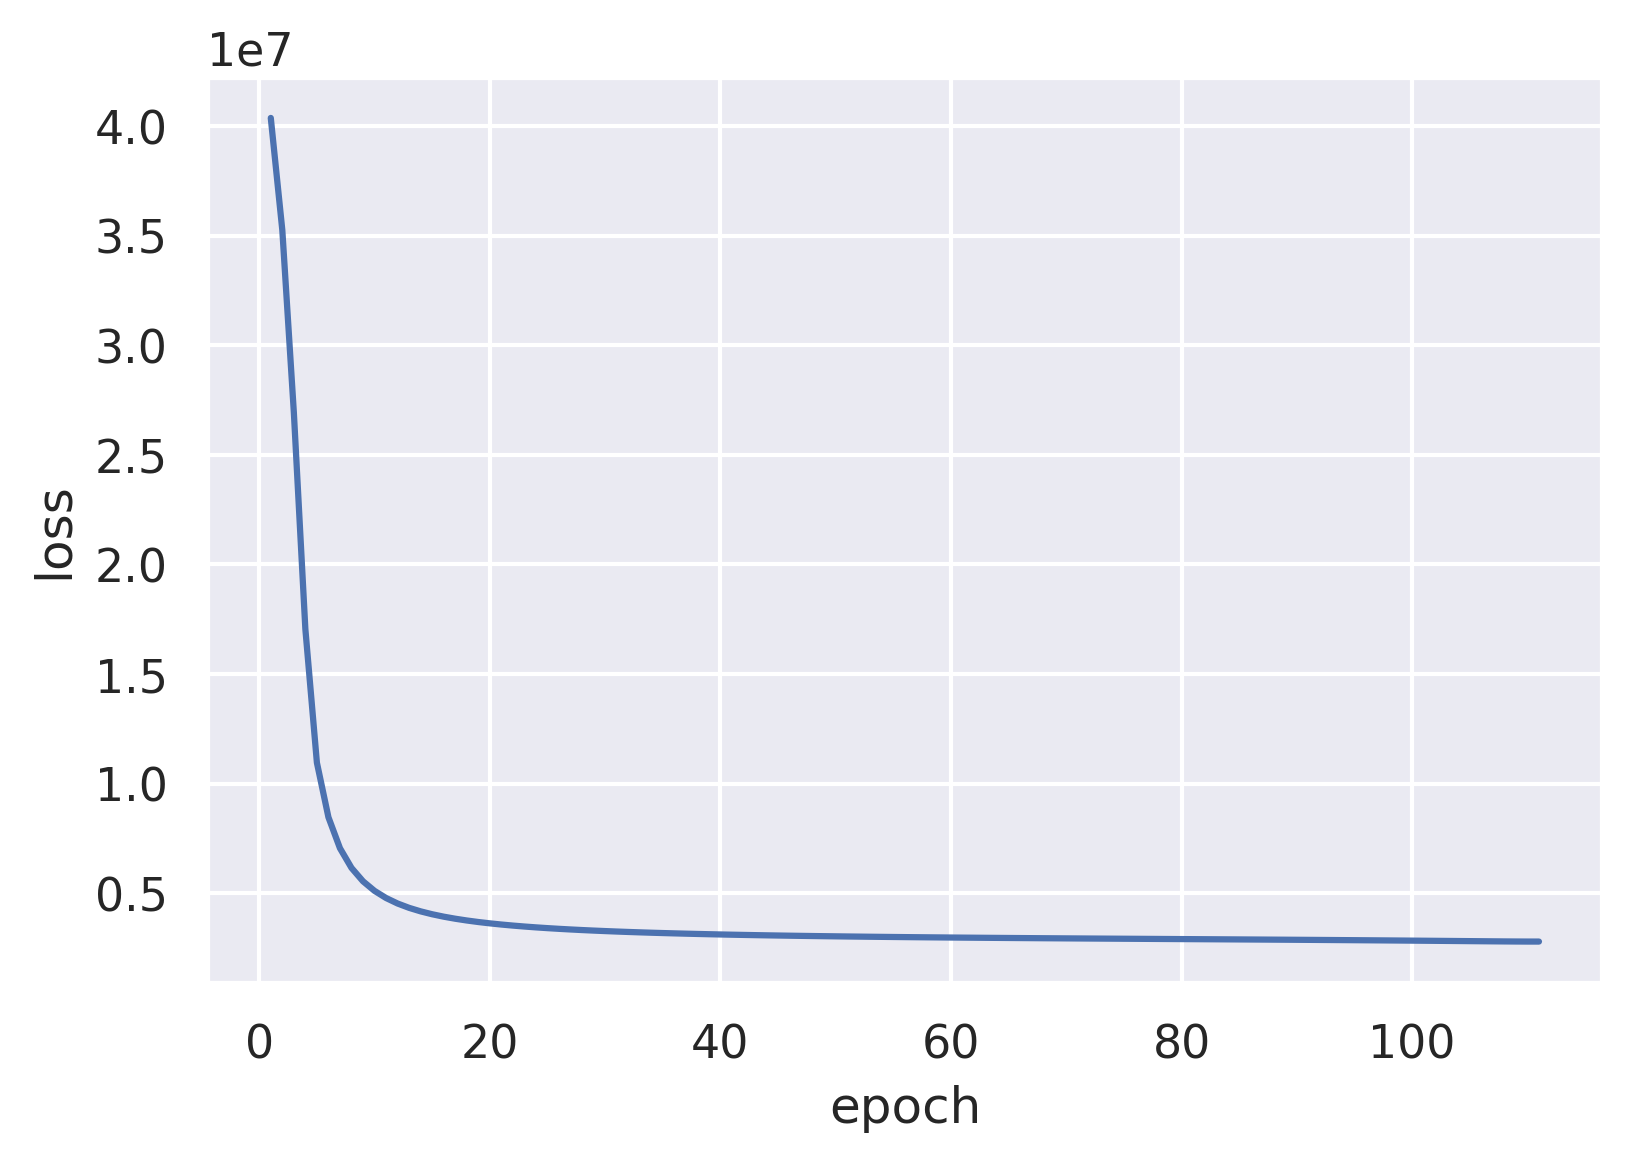
\includegraphics[width=.5\linewidth]{bigdata_loss.png}}%
\hspace{4em}%
\subcaptionbox{测试集 RMSE\label{fig:rmse}}
{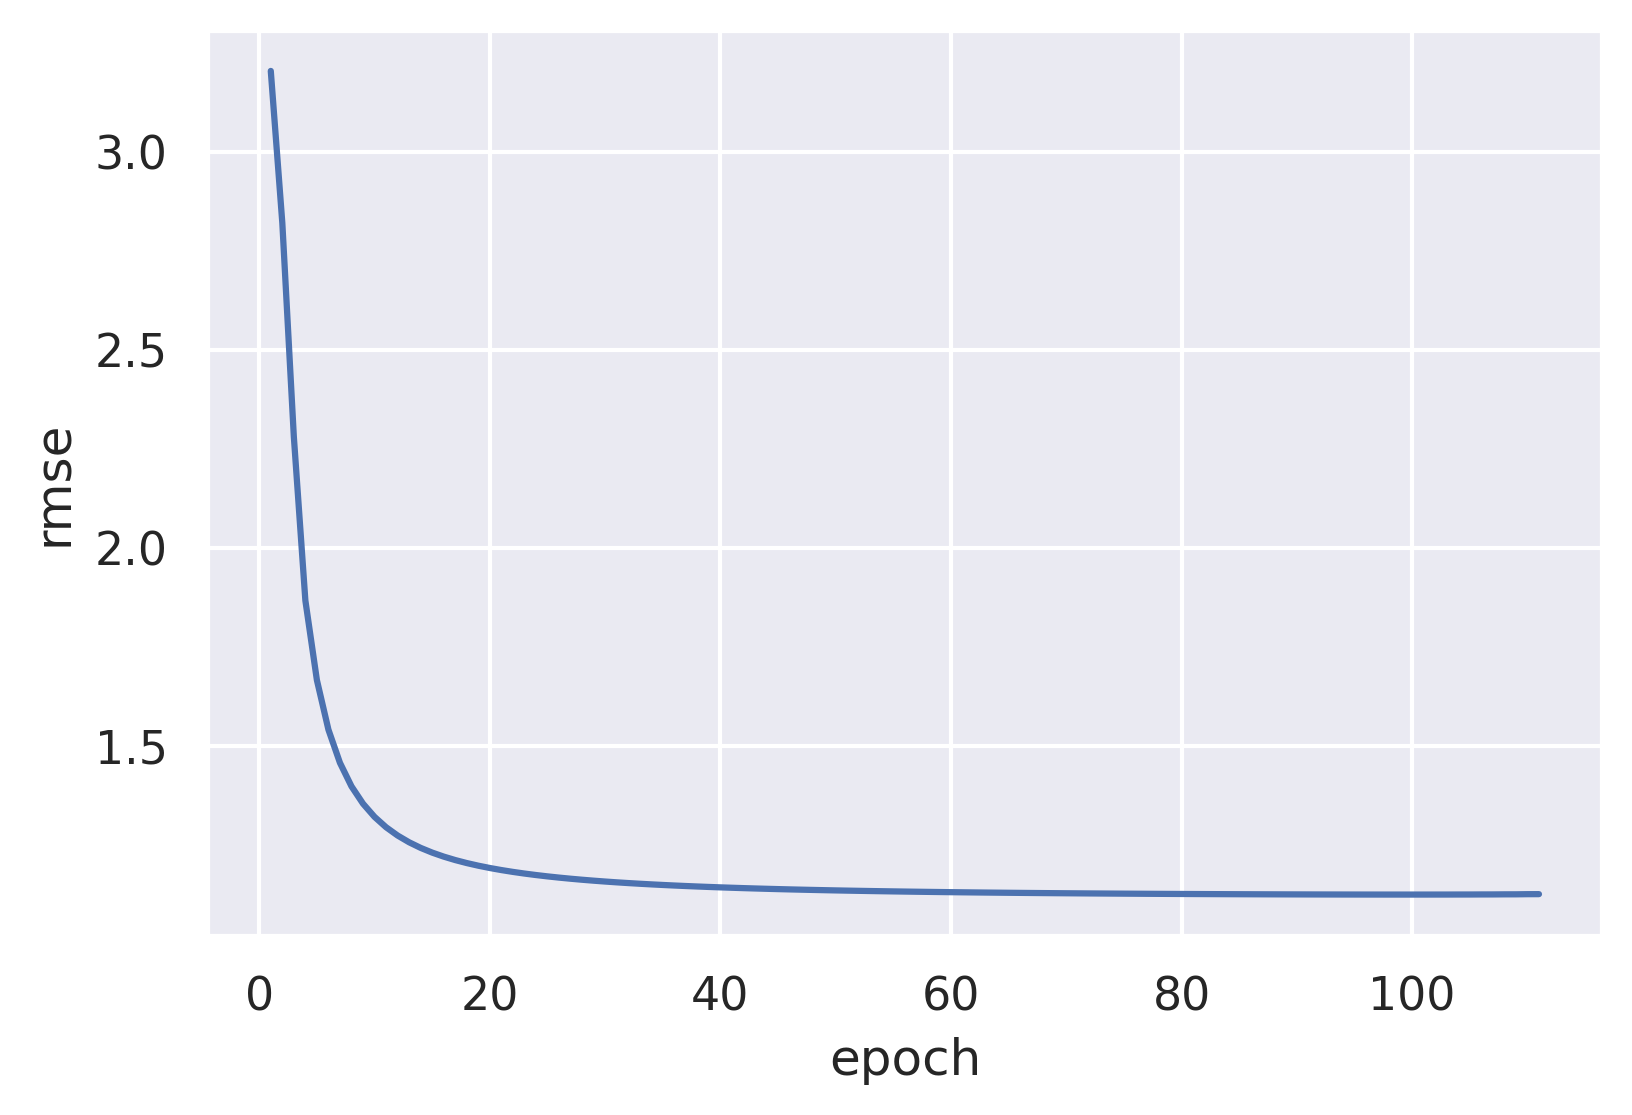
\includegraphics[width=.5\linewidth]{bigdata_rmse.png}}
  \caption{迭代过程中的训练和测试误差}
  \label{fig:training}
\end{figure}

如图\ref{fig:training} 所示,训练损失值和测试误差(RMSE)变化都是稳定下降的,并且下降幅度随着训练代数的增加逐渐减小。
因为训练和测试用的损失值公式不一样,所以可以看出,训练的时候,损失值都很大,不过到了测试的时候,损失值是比较小的。
采用 EarlyStop 技巧,超参数设置为 $\alpha=0.0001, \lambda = 0.01, k=50$,最终训练了 111 代后的测试结果 RMSE 为 $1.12452$,总共耗时 $31.86$s。

\section{寻找最优超参}

$k$ 选择 $\{10, 20, 30, 50\}$, $\lambda$ 选择 $\{0.001, 0.1, 0, 10\}$,学习率 $\alpha$ 使用 $0.0001$,最大训练代数为 $400$,采用 EarlyStop。
进行 GridSearch 最优的超参数配置,不同参数的训练损失值曲线如图所示,最终的测试 RMSE 结果如表所示。

从实验结果可以看出,

\chapter{总结:}

协同过滤:

\begin{enumerate}
  \item \textbf{可解释性好}:因为公式简单明了,算法的思路就是从当前用户行为特征(例如打分向量)相似(通过某种相似度衡量)的其他用户的打分分数来预测该用户对指定电影的打分情况。
  \item \textbf{算法稳定}:对于给定的输入,不管运行多少次,都能得到相同的结果。
  \item {优化空间小}:因为这是一种无参方法,只能通过使用不同的相似度量,不同的邻域函数(例如 kNN),不用的聚合函数来实现,这些选择与具体任务相关,都需要专家经验。
\end{enumerate}

矩阵分解:

\begin{enumerate}
  \item \textbf{灵活性强}:可以配合使用各种不同的目标函数。
  \item \textbf{适合显卡并行运算}:使用 CuPy 等显卡加速矩形计算工具的计算速度提升明显。
  \item {泛化性好}:因为可以通过梯度优化以及调整超参数,所以对于不同任务,不用做额外的修改。
  \item {可解释性不好}:因为基于低秩假设,且隐特征的解释性不好,算法通过梯度下降寻找在给定目标函数下的局部最优解。
  \item {超参数调整费时}:因为可解释性不好,所以对于超参数 $\lambda, \alpha, k$ 的调整都只能结合一点调参经验,遍历搜索,比较费时,而且不同任务适合的超参数也不一样。
\end{enumerate}

\textbf{注:} 矩阵分解其实是一种协同过滤算法,(广义的)协同过滤是一种思想而不是特定的某个算法。

% 其他部分
\backmatter

% 参考文献
\bibliography{ref/refs}  % 参考文献使用 BibTeX 编译

% 附录
\appendix
\end{document}
